\documentclass[../main.tex]{subfiles}

\begin{document}

\theoremstyle{definition}
\newtheorem{Def}{Définition}

\theoremstyle{plain}
\newtheorem{Conj}{Conjecture}

    \label{sec:test2}
    Dans cette section, nous allons vérifier si des conjectures sur les nombres premiers peuvent s'appliquer aux ensembles aléatoires créés à la section \ref{sec:sec1}. Ainsi, on sera en mesure d'estimer si la véracité d'une conjecture est susceptible de tenir grâce à la répartition des nombres premiers plutôt qu'à leur propriété d'être premier. 
 
 \subsection{Les nombres premiers jumeaux} 
 \subsubsection{Introduction}
 	La première conjecture que nous allons analyser, et sans doute la plus célèbre, est la conjecture des nombres premiers jumeaux.
	\begin{Def}
	Soient $a$, $b \in \mathbb{N} $, $ a < b$, on dit que $a$ et $b$ sont jumeaux si $ a + 2 = b $.
	\end{Def}  
	
	\begin{Conj}
	Il y a une infinité de nombres premiers jumeaux.
	\end{Conj}
	
	Ces dernières années, il y'a eu de grosses avancées dans la démonstration de la conjecture (voir l'article~\cite{article_polymath}). Ainsi, pour tout $ m \geqslant 1$, soit $H_{m} := $ $\liminf_{n \rightarrow \infty}  (p_{n+m} - p_{n})$, où $p_{n}$ dénote le n-ième nombre premier. La conjecture des nombres premiers jumeaux est donc équivalente à $H_{1} = 2$. En 2013, le mathématicien chinois Zhang Yitang est le premier à trouver une borne supérieure finie pour $H_{1}$, il a démontré que $H_{1} \leqslant 70\, 000\, 000$. Suite à la publication de Zhang Yitang, de nombreux mathématiciens se sont mis en quête de réduire la borne supérieure de $H_{1}$. En optimisant les résultats de Zhang Yitang et grâce à d'autres méthodes ils ont pu montrer que $H_{1} \leqslant 246$.

\subsubsection{Analyse}
	Afin de tester la conjecture sur les ensembles aléatoires, nous avons tracé un graphe (figure \ref{im:image4}), où pour chaque ensembles aléatoires et l'ensemble des nombres premiers (jusqu'à $10^{7}$) on trace une fonction qui compte le nombre de jumeaux.
\begin{figure}[H]
 \centering
 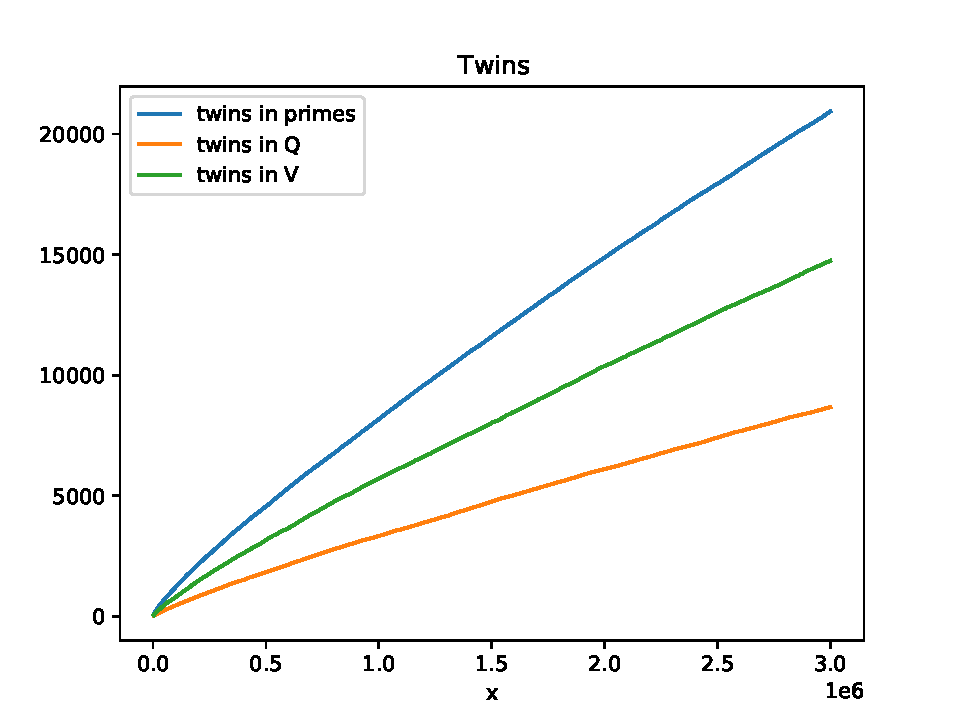
\includegraphics[keepaspectratio=true, width=12cm]{twins.pdf}
 \caption{Nombre de jumeaux dans chaque ensemble}
 \label{im:image4}
 \end{figure}
 
 \newpage
 
 Nous pouvons faire les observations suivantes : 
 	\begin{itemize}
	\item Pour chaque type d'ensemble (selon l'approche utilisée), on constate, logiquement, que le nombre de jumeaux est plus ou moins le double pour les ensembles impairs;
	\item Il y'a plus de jumeaux dans les ensembles $R$ que dans les ensembles $Q$, ce qui est probablement dû à la construction des ensembles;
	\item De manière générale, toutes les courbes sont croissantes, ce qui indiquerait, autant pour les nombres premiers que pour les ensembles aléatoires, que le nombre de jumeaux tend vers l'infini. 
	\end{itemize}
	
	Par ailleurs, ce graphe éveille deux idées intéressantes qui prouveraient la conjecture. Soient $ f : [2, \infty[ \rightarrow \mathbb{R}, x \mapsto \# \{ n \in \mathbb{P}$ | $n+2 \in \mathbb{P}$ et $n+2 < x  \}$  ($\mathbb{P}$ désigne ici l'ensemble des nombres premiers) et $ g : [2, \infty[ \rightarrow \mathbb{R}, x \mapsto \# \{ q \in Q$ | $n+2 \in Q$ et $q+2 < x  \}$, où $Q$ est un ensemble aléatoire quelconque. Alors :
\begin{itemize}
	\item Si $f(x) \sim g(x)$ quand $x$ tend vers l'infini et $\lim\limits_{x \rightarrow +\infty} g(x) = \infty$ alors $\lim\limits_{x \rightarrow +\infty} f(x) = \infty$. Pour ce faire une idée d'une éventuelle similarité entre $f$ et $g$ quand $x$ tend vers l'infini, nous avons tracé le graphe de $\frac{f(x)}{g(x)}$ (figure \ref{im:image6});
	\item Si $f \geqslant g$ et $\lim\limits_{x \rightarrow +\infty} g(x) = \infty$ alors $\lim\limits_{x \rightarrow +\infty} f(x) = \infty$.
\end{itemize}
\begin{figure}[H]
 \centering
 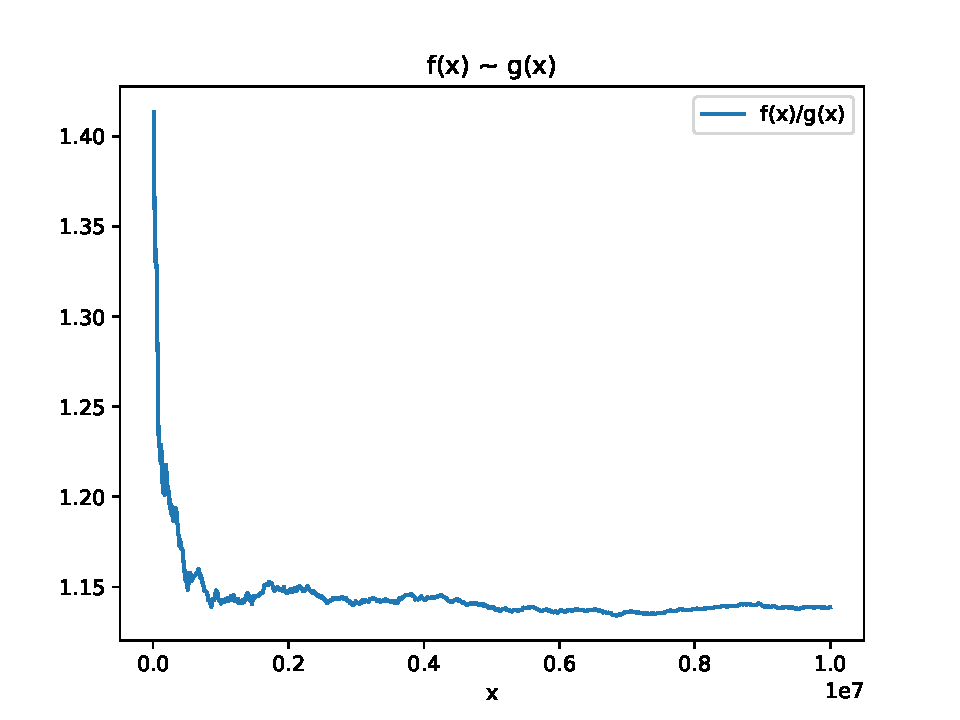
\includegraphics[keepaspectratio=true, width=12cm]{ecarts_count_twins.pdf}
 \caption{$\frac{f(x)}{g(x)}$}
 \label{im:image6}
 \end{figure}


	De plus, pour les ensembles aléatoires $R$ (créés selon l'approche probabiliste), on peut avoir une bonne approximation de la fonction $g$. Soit $R$ un tel ensemble, on définit $ h : [0, \infty[ \rightarrow \mathbb{R}, x \mapsto \sum_{i = 2}^{\lfloor x \rfloor}  \frac{1}{\log(i) \log(i+2)}$. Par construction, pour $i \geqslant 3$, la probabilité que $i \in R$ vaut $P(i \in R) = \frac{1}{\log(i)}$. Donc, la probabilité que $i$ et $i+2 \in R$ vaut $ P(i \in R $ et $i+2 \in R) = \frac{1}{\log(i)\log(i+2)}$. En additionnant les probabilités, on obtient l'espérance mathématique. À titre comparatif, voici le graphe de $h(x)$, $f(x)$ et $g(x)$ (figure \ref{im:image7}).
\begin{figure}[H]
 \centering
 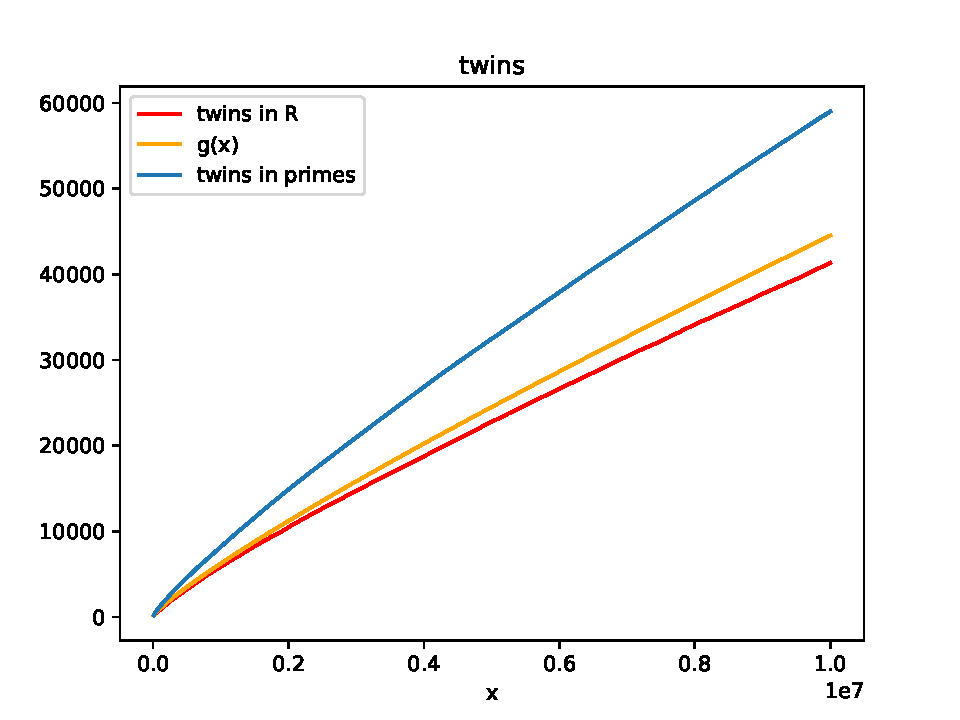
\includegraphics[keepaspectratio=true, width=12cm]{comparaison_twins.pdf}
 \caption{Comparaison de $h(x)$ avec $g(x)$ et $f(x)$}
 \label{im:image7}
 \end{figure}
On peut montrer que $\lim\limits_{x \rightarrow \infty} h(x) = + \infty$ et ainsi prouver l'infinité des jumeaux dans un ensemble $R$, en supposant l'ensemble infini. 

\subsubsection{Conclusion de l'analyse}
Pour conclure, nos méthodes de constructions d'ensembles aléatoires semblent, comme pour les nombres premiers, avoir une infinité de nombres jumeaux tout en ayant des résultats très différents entre les différents types d'ensembles. Ceci est probablement dû à la construction des ensembles. En effet, par l'approche analytique, pour le choix du n-ième élément on impose une distribution uniforme parmi un nombre fixe de possibilités. Tandis que pour l'approche probabiliste, le choix de l'élément $n$ ne dépend que de la probabilité $\frac{1}{\log(n)}$, ce qui nous permet d'avoir une bonne approximation de la fonction $g$, la fonction $h$. 

\clearpage
\end{document}




